\section{Continuous Training and Serving} \label{continuous-training-serving}
The underlying optimization algorithm we utilize for continuously training the deployed model is Stochastic Gradient Descent (SGD).
Using SGD enables us to make frequent updates to the model, thus increasing the quality and the freshness of the deployed model.
SGD algorithm has several parameters and in order to work effectively, they have to be tuned.
In this section, we first describe the details of SGD and its parameters and our approach in tuning these parameters for our platform.
Then we describe how we take advantage of the properties of SGD to implement our proactive training, online statistics computation, and data materialization.
Another important aspect of any deployment platform is the ability to monitor the quality of the deployed model.
We present our method for evaluating the quality of the deployed model and how we guarantee high-quality models.
In the last part of this section, we describe how utilizing our continuous training approach improves the efficiency of online advertising example described in Section \ref{introduction}.

\subsection{Stochastic Gradient Descent} \label{sgd}
\textit{Stochastic Gradient Descent (SGD)} is an optimization strategy utilized by many machine learning algorithms for training a model.
SGD is an iterative optimization technique where in each iteration, a sample of the data is used to make updates to the model.
SGD is suitable for large datasets as it does not require scanning the entire data in every iteration \cite{bottou2010large}.
SGD is used in different machine learning tasks such as classification \cite{zhang2004solving, macmahan2013}, clustering \cite{bottou1995convergence}, and matrix factorization \cite{koren2009matrix,  funk2006netflix}.
It is also widely used in neural networks for training the networks on large datasets \cite{dean2012large}.
Prominent applications of SGD in neural networks are the work of Google Deepmind team that managed to train neural networks that defeat humans in the game of Go \cite{silver2016mastering} and mastering Atari games \cite{mnih2013playing}.

In our example application, a logistic regression model is trained using the SGD optimization method \cite{macmahan2013}.
In logistic regression, the goal is to find the weight vector ($w$) that maximizes the conditional likelihood of labels ($y$) based on the given data ($x$) in the training dataset:

\begin{center}
$w^* = \argmin_w ln(\prod_{i=1}^{N} P(y^i | x^i, w))$
\end{center}

where $N$ is the size of the training dataset.
To use SGD to find the optimal $w$, we start from initial random weights and in each step make small updates based on the gradient of the loss function:

\begin{center}
${w}^{t+1} = {w}^t + \eta \sum_{i \in S} x^i (y^i - \hat{P}(Y^i = 1 | x^i w))$
\end{center}

where $\eta$ is the learning rate parameter and $S$ is the random sample in the current iteration.
The algorithm continues until convergence (when the weight vector does not change after an iteration).

\textbf{Learning Rate.}
A very important parameter of stochastic gradient descent is the learning rate.
The learning rate controls the degree of change in the weights in each iteration of SGD.
The most basic approach of tuning the learning rate is setting it to an initial small value and after each iteration decrease the value by a small factor.
In complex and high-dimensional problems, this simple tuning approach for the learning rate is not effective \cite{schaul2013no}. 
Adaptive learning rate methods such as, Momentum \cite{qian1999momentum}, Adam \cite{kingma2014adam}, RMSPROP \cite{tieleman2012lecture}, and AdaDelta \cite{zeiler2012adaptive} have been proposed.
These methods automatically adjust the learning rate value in every iteration and speed up the convergence time.
Moreover, some of the adaptation methods perform per coordinate modification \cite{schaul2013no, tieleman2012lecture, zeiler2012adaptive}. 
This is important because not all the parameters of the weight vector contribute the same way and some of the parameters change more rapidly during the training process.

\textbf{Sample Size.}
Another parameter of stochastic gradient descent is the sample size.
SGD is guaranteed to converge to a solution regardless of the sample size.
However, the sample size can greatly affect the time that is required to converge.
Two extremes of the sample size are 1 (every iteration only considers 1 data item) and $N$ (every iteration consider the entire data set, similar to normal batch gradient descent).
Setting the sample size to 1 increases the model update frequency, however, it also results in noisy updates.
Therefore, more iterations are required for the model to converge.
Using the entire data in every iteration leads to more stable updates and as a result, the number of iterations required for the model to converge is fewer.
However, each iteration takes more time as more data has to be processed.
The most common approach is to set the sample size to a value small enough so that each sample can be processed quickly but large enough so the updates are not noisy (called a mini-batch gradient descent).

\textbf{Distributed SGD.}
To efficiently train machine learning models on large datasets, scalable techniques have to be employed.
SGD inherently works well with large amounts of data because it does not need to scan every data point during every iteration.
However, for very large datasets, SGD has to perform many iterations in order to converge.
To decrease the running time, large datasets can be distributed among multiple nodes, where each node will compute the gradients on a subset of the data in parallel.
After the initial computation of the gradients, they are all sent to one node where the final gradients are computed.

\subsection{Proactive Training}
We use the iterative nature of SGD in the design of our continuous training process.
After the initial model is deployed, new iterations of SGD can be performed on a combination of the existing and new data.
Once the gradients are computed, we update the deployed model.
However, the two parameters of SGD (learning rate and sample size) play an important role.
They have to be tuned to increase the efficiency of the training.
Choosing  a very small sample size may result in inaccurate updates and as a result, degrade the quality of the deployed model.
On the other hand, a very large sample size leads to a lengthy training process and less frequent model updates.
Similarly, learning rate should be adapted accordingly.
We view proactive training as an extension of the offline batch training.
Therefore, the process of choosing the best sample size and learning rate adaptation technique is similar to static training.
Different hyperparameter tuning techniques are proposed for finding the best set of hyperparameters.
Most common and simplest approaches are grid search and random search \cite{bergstra2012random}.
We use a grid search over the initial training data to find the best hyperparameters (in our system, learning rate adaptation technique and sample size).
Once the initial model is trained and deployed, the same set of parameters are used for the proactive training.

\textit{Scheduling rate.}
An extra parameter of proactive training is the scheduling rate.
In offline training, iterations of SGD are executed one after the other until convergence.
In proactive training, the scheduling rate defines the frequency of SGD iteration execution.
The scheduling rate plays an important role as it directly affects the freshness of the deployed model.
However, a high scheduling rate results in many frequent SGD iterations which incur an overhead on the deployment system as it is using a lot of resources.
A small scheduling rate also affects the model freshness.
To increase the efficiency of the system a scheduler component is designed that is tasked with scheduling new iterations of SGD.
Similar to learning rate tuning, we use an adaptive approach to adjust the scheduling rate.
We describe a method for tuning the scheduling rate based on the rate of the incoming training data.
The scheduling rate is increased as the rate of the incoming training data increases and vice versa.
This helps in adapting the model to the new training data.

\subsection{Online Statistics Computation and Data Materialization}
Before training the machine learning model, the training dataset has to be processed by the pipeline.
Different components of the pipeline require statistics over the dataset to be calculated before they process the data.
Computing these statistics require scans of the data.
In our deployment platform, we provide a mechanism for online computation and update of the statistics required for different components of the pipeline.
In our prototype, we implemented a standard scaler, a missing value imputer, and a one-hot encoder.
The above components require the mean, the standard deviation, and for the one-hot encoder, the hash table of the unique categorical parameters in every feature column.
Our deployment platform also accommodates custom pipeline components.
When new training data arrives at the system, the platform directs the data to the corresponding component so they update their underlying statistics and data structures.
Computing the required statistics online reduces the model training time as computing these statistics offline is time-consuming.
Every pipeline component needs to transform the data when it is updating its statistics.
The component then passes the transformed data to the next component.
Once every pipeline component updates their statistics, the resulting transformed data is ready for model training.
We provide an optional feature that allows materialization and storage of the transformed data on disk.
As a result, during the next SGD iterations, the system skips the preprocessing steps of the pipelines and directly accesses the transformed data to train the model.
Storing the transformed data significantly reduces the model training time.

\textit{Dynamic model size.}
Depending on the type of the pipeline components, the size of the final model may need to be adjusted during the serving of the model.
For example, one-hot encoding and \hl{data bucketization} both may generate new features after processing new training data.
After every statistics update, we analyze the changes made in the pipeline.
If any of the changes result in an increase in the model size, we dynamically adjust the model size in the next proactive training. 

\subsection{Model Stability}
\begin{figure}[t]
\centering
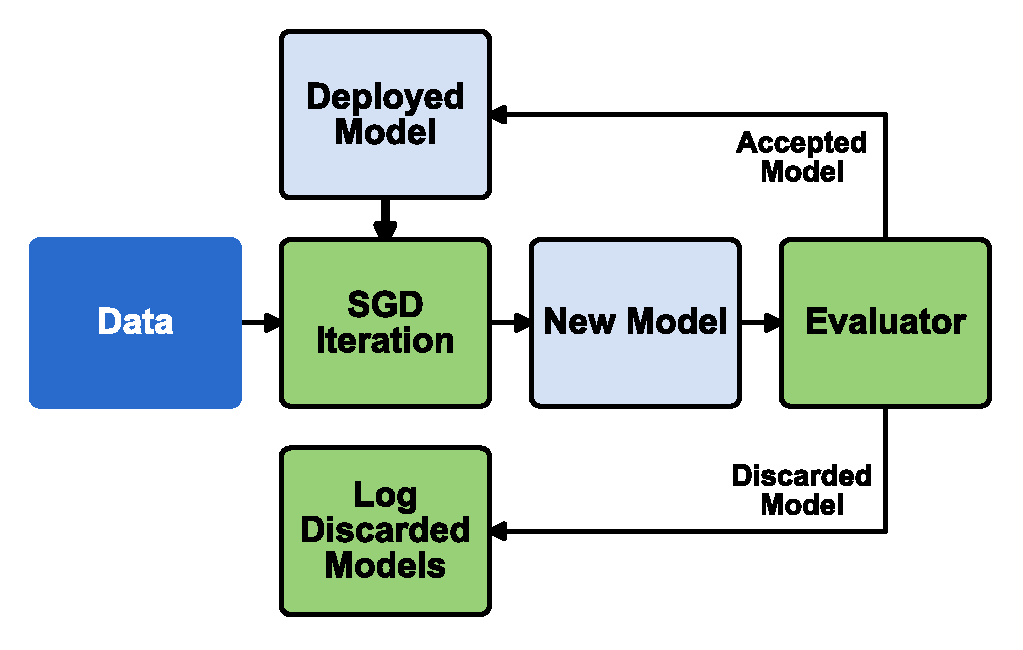
\includegraphics[width=\columnwidth]{../images/model-evaluation.pdf}
\caption{Model Evaluation}
\label{fig:model-evaluation}
\end{figure}

To ensure that SGD iterations do not degrade the quality of the model, a model evaluator is used to assess the quality of the model.
Figure \ref{fig:model-evaluation} shows the process of model evaluation.
Every iteration of the SGD, uses the latest deployed model as an initial starting point and updates the model based on the training data.
The evaluator assesses the quality of the model using an evaluation dataset.
If the quality of the model has degraded, the update is discard and the model is logged.
The engineers or administrators of the system can study the log in order to investigate any potential issues with machine learning pipeline or the incoming training data.

\subsection{Improved Example Application}
\begin{figure}[t]
\centering
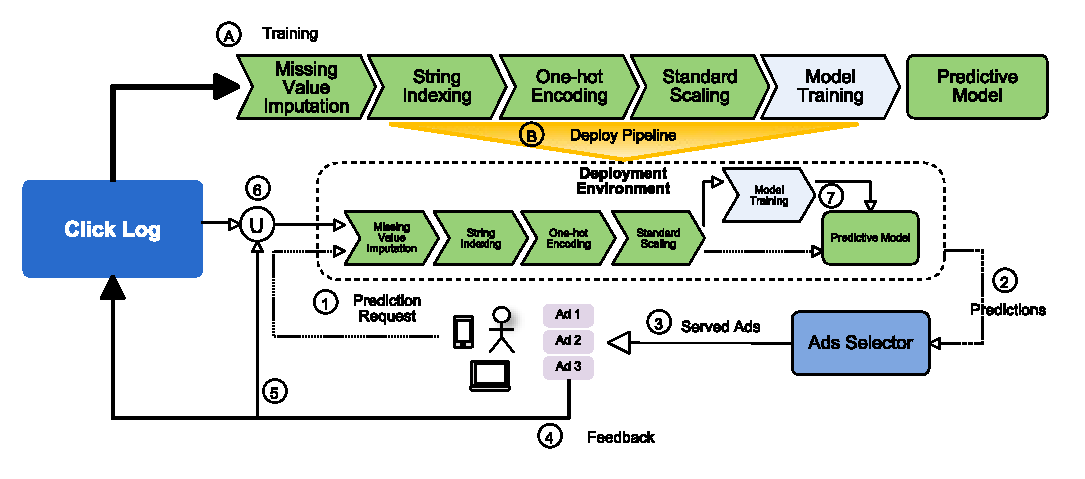
\includegraphics[width=\columnwidth]{../images/improved-example.pdf}
\caption{Ads Serving Continuous Training}
\label{fig:improved-example}
\end{figure}

Figure \ref{fig:improved-example} shows how our deployment approach improves the example application described in Section \ref{introduction}.
After the training of the initial model \textcircled{A}, the model and the pipeline are deployed to the deployment environment \textcircled{B}.
Prediction requests are sent by the user to the deployment environment \textcircled{1} where based on the current model for each ad a score is predicted \textcircled{2}.
Based on the score a few ads are shown to the user \textcircled{3}.
Depending on whether or not the user clicks on them, feedback is sent back to the deployment system \textcircled{4}.
Similar to current approaches the data is stored in the click log database.
However, contrary to the existing methods, the data is routed to the deployment platform immediately.
The deployment platform forwards the training data to the pipeline components to compute the required statistics \textcircled{5}.
The deployment platform periodically samples the historical data \textcircled{6}.
Based on this sample and the new training data, an iteration of SGD is performed which updates the deployed logistic regression model.
If the new model is accepted, it is redeployed \textcircled{7}.
New prediction requests that arrive at the system will be answered by the new model.
In the new workflow, the deployment platform continuously updates the pipeline and the deployed model without requiring a full retraining over the click log dataset.
The deployment platform ensures that the model is always up-to-date and the information about new users or new ads are taken into account in the next iteration of stochastic gradient descent.
This increases the model freshness without affecting the model quality.